\frontmatter
\title{Matroid Theory}
\author{Héctor Manuel Téllez Gómez}
\date{January 27, 2014 - \today}
\maketitle

\tableofcontents

\mainmatter
\chapter*{Note for the readers:}
    The goal on writing this in english instead of writing it in my first language (spanish) is because 
    this way I can start building a portfolio that could not be as important as a research project, but
    it is work after all. So it would be better to have something to show that nothing to show at all, 
    and much better if the audience capable of read it is as wide as possible.\pn
    
    As my first language is not english, this text could have a lot of mispellings and
    bad use of english. I apologize in advance and I'll try to be as careful as possible.\pn
    
    Here is a link to this project's version controller repository:\par
    \href{https://github.com/tellezhector/matroids}{https://github.com/tellezhector/matroids}\par
    There you can see what are the changes that have ocurred along all this project's lifetime.\pn
    
    If you want to leave comments you can do it there, where anyone else is able to notice it. Or you could 
    write directly to my personal e-mail address, which is: \texttt{tellez.hector@gmail.com} where it will be read only
    by me.

\chapter{Union Of Closed Sets That Is Not Closed}
\begin{definition}[Closure]
    Given a matroid $M=(E,\c{J})$ with rank function $f$. The \textbf{closure} of a set $S \subset E$
    is
    \begin{align}
        Cl(S) = \{ x \in E | r(S \cup \{ x \} ) = r(S)\}.
    \end{align}    
\end{definition}

\begin{definition}[Closed set]
    Given a matroid $M=(E,\c{J})$ with rank function $f$. We say that a set $S \subset E$ is \textbf{closed}
    if
    \begin{align}
        Cl(S) = S.
    \end{align}
\end{definition}

\prob
{
    Give an example of two closed sets whose union is not closed.
}

\begin{proof}
    We are going to use the linear matroid of $\Z^2$, where the independent sets are 
    $$\emptyset, \{(1, 0)\}, \{(0, 1)\}, \{(1, 1)\}, \{(1, 0), (0, 1)\}$$
    and the rank function is the size of the biggest independent set contained.\pn
    
    It is clear that $A = \{(1, 0), (0, 0)\}$ and $B = \{(0, 1), (0, 0)\}$ are both closed.
    But $C = A \cup B = \{(1, 0), (0, 1), (0, 0)\}$ is not, because $r(C) = 2 = r(C \cup \{ (1, 1) \})$ and
    $(1, 1) \not\in C$.
\end{proof}

\chapter{First Test}
    \begin{center} February 17, 2014 \end{center}
    Test for Oxley's book first chapter (Basic definitions and examples). 
    
    \section{Problem 1 (Oxley, Section 1.1, Problem 2)}
        \prob{
    Let A be the matrix
    $$\bordermatrix{
            &   1   &   2   &   3   &   4   &   5   &   6   \cr
            &   1   &   0   &   0   &   1   &   1   &   0   \cr
            &   0   &   1   &   0   &   1   &   0   &   1   \cr
            &   0   &   0   &   1   &   0   &   1   &   1   
    }$$

    For q in $\{2,3\}$, let $M_q[A]$ be the vector matroid of $A$ when $A$ is viewed over $GF(q)$,
    the field of $q$ elements. Show that:

    \begin{enumerate}
        \item[(i)] 
            The sets of circuits of $M_2[A]$ and $M_3[A]$ are different.
        \item[(ii)]
            $M_2[A]$ is graphic but $M_3[A]$ is not.
        \item[(iii)] 
            $M_2[A]$ is represntable over $GF(3)$, but $M_3[A]$ is not representable over $GF(2)$.
    \end{enumerate} 
}

\begin{proof}\label{t1:p1}
    \begin{enumerate}[label=(\roman*)]
        \item\label{t1:p1i}
            Lets look for the circuits over $GF(2)$. As $0$ and $1$ are the only scalars over $GF(2)$,
            we can only pay attention to sums of the vector columns and forget about full linear combinations.\pn
            
            There are no loops, the only way to get a loop is having a zero column and it is not the case.\pn
            
            There are no circuits of length two (or parallel columns), the only way to get them is having two 
            exactly equal columns and it is not the case.\pn
            
            Lets call the columns 1, 2, and 3 the ``simple columns'', and the columns 4, 5 and 6 the ``double columns''.\pn
            
            For any pair of the columns from the simple columns there is a column from the double columns 
            such that the sum is zero. Such column is the one you can get from adding the chosen pair. 
            That is, $\{1, 2, 4\}$, $\{1, 3, 5\}$, $\{2, 3, 6\}$ are three dependent sets.\pn
            
            If you try to add all the simple columns, you can't add up to zero.\pn
            
            If you add two of the the double columns, you get the third one, so $\{4, 5, 6\}$ is dependent.\pn
            
            These four sets are circuits given that there are no smaller dependent sets.\pn
            
            These four are all the circuits of size three. Lets think about the circuits of size four.\pn
            
            Again, if you add two of the double columns, you get the third one, and there are two simple columns that can
            add up this third one. So, $\{1, 2, 5, 6\}$, $\{1, 3, 4, 6\}$, $\{2, 3, 4, 5\}$ are dependent sets.
            And no one of the four already given circuits are contained in them, so these are circuits themselves.\pn
            
            At any time you choose the three simple columns, you will get no way to add up to zero just adding double columns.
            So, any set containing all of the simple columns will not be a circuit.\pn
            
            If you choose all the double columns, you have already chosen a circuit, so if you add any other vector,
            you will get a dependent set that is not a circuit.\pn
            
            So these seven are all the circuits of $M_2[A]$.\pn
            
            Now lets look for the circuits over $GF(3)$. Again and for the same reason, there are not loops or parallel columns.\pn
            
            If you choose two simple colums and you add them, you get one of the double columns, so if you add to them the
            negative of this double column, you get the zero vector. So $\{1, 2, 4\}$, $\{1, 3, 5\}$, $\{2, 3, 6\}$ are
            circuits.\pn
            
            $\{4, 5, 6\}$ is not dependent, you can check that the determinant of their submatrix is $2$ (or -2 if you switched
            something).\pn
            
            If you choose two doble columns and add to them a simple one, again the determinant is not zero (it is always 1 or -1).
            So $\{1, 2, 4\}$, $\{1, 3, 5\}$, $\{2, 3, 6\}$ are all the circuits of size three.\pn
            
            Now lets look for circuits of size four.\pn
            
            If you choose two double columns and add one to the negative of the second one, you can find two simple columns that 
            can make them add up the zero vector (using the correct signs), these two vectors are exactly the ones that add up to
            the double column that you didn't choose. So none of these selections contains the circuits of size three and therefore
            they are circuits. So this give us the circuits $\{1, 2, 5, 6\}, \{1, 3, 4, 6\}, \{2, 3, 4, 5\}$.\pn
            
            If choose all of the double columns, you can choose any of the simple one so the four of them add up the zero vector using
            an appropiate selection for the signs. So this give us the dependent sets $\{1, 4, 5, 6\}, \{2, 4, 5, 6\}, \{3, 4, 5, 6\}$ 
            and they are circuits because any of the smaller circuits contain at least two simple columns.\pn
            
            The only other chance is choosing all of the simple columns, but wathever you add, you will get any of the three sized
            circuits as a subset. So these six are all of the circuits of size four.\pn
            
            There are no circuits of size five, because there are only two posibilities, having three simple columns and two double columns, 
            or having three double  columns and two simple columns. The first one, again contains as a subset a circuit of size three.
            The second one always contains as a subset a circuit of size four.\pn
            
            So in total, there are nine circuits for $M_3[A]$.\pn
                        
            Only by their cardinality, you can tell that the set of circuits of $M_2[A]$ and $M_3[A]$ are different.
            
        \item\label{t1:p1ii}
            We are going to give a graphic representation of a graph that has $M_2[A]$ as an isomorphic matroid. You can
            verify that it has all the seven circuits that we gave previously and only those.\pn

            \begin{figure}[H]
                \centering
                    \caption{}
                    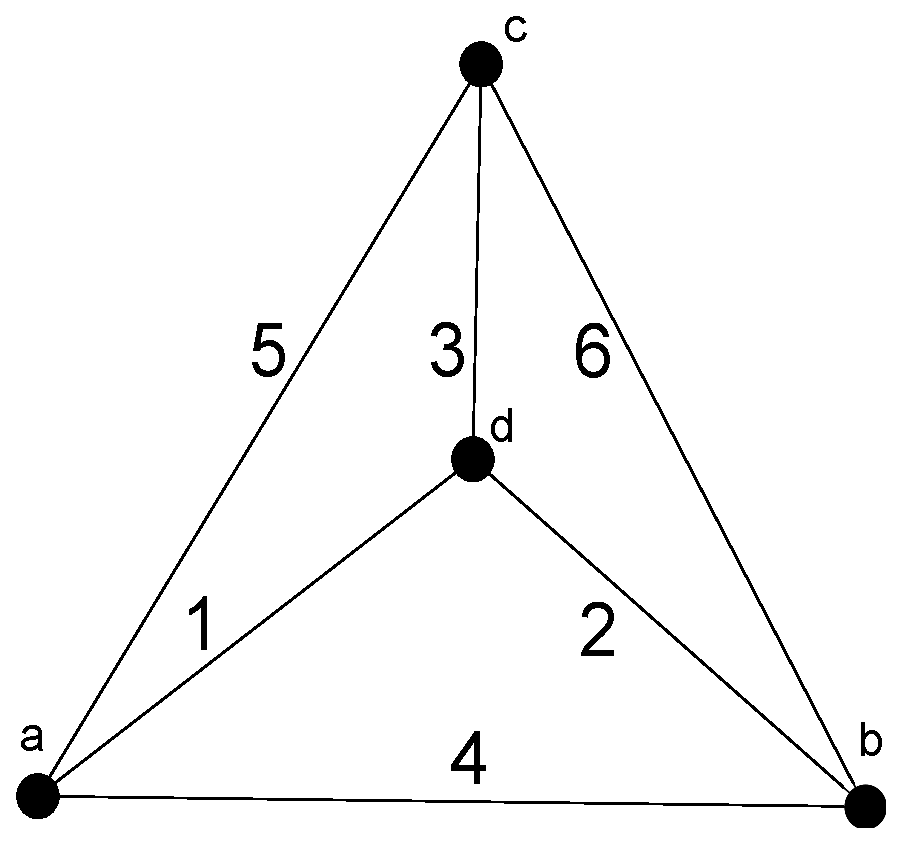
\includegraphics[width=6cm]{Test1/Problem1/tetrahedron.eps}
                \label{fig:tetrahedron}
            \end{figure}
            
            Now lets think what could happen if $M_3[A]$. For $M_3[A]$, we have the circuits 
            $\{1, 4, 5, 6\}, \{2, 4, 5, 6\}, \{3, 4, 5, 6\}$. Take any two of them, lets say
            $\{1, 4, 5, 6\}, \{2, 4, 5, 6\}$, they have three edges in common $\{4,5,6\}$. \pn
            
            If there is a graphic mathroid isomorphic to $M_3[A]$, $\{4,5,6\}$ defines three edges of a 
            $4$-cycle, that is, a $3$-trajectory. In any $3$-trajectory we will find $4$ vertices, so the fourth 
            edge is already determined by two of those vertices (the start vertex and the last vertex), but in this case 
            we have that $\{1, 4, 5, 6\}$, $\{2, 4, 5, 6\}$ are both $4$-cycles over the same set of vertices, 
            and so $1$ and $2$ have exactly the same two vertices, that is, they are parallel. But in [\ref{t1:p1}.\ref{t1:p1i}]
            we saw that $M_3[A]$ has no parallel columns. So this is a contradiction.
        
        \item\label{t1:p1iii}
            We are going to give a matrix $B$ over $GF(3)$ such that $M_3[B]$ isomorfic to $M_2[A]$.\pn
            
            We are going to take the incidence matrix for the graphic representation [\ref{fig:tetrahedron}], and
            choose one ``1'' from each column and change it by ``-1''. What we are doing is giving a orientation
            to each of the edges. So, if a cycle is such that each edge has exactly outdegree 1 and indegree 1, is
            easy to see that the sum of the respective columns will be the zero vector (each 1 will have exactly one -1 in
            its same row).\pn
            
            But lets remember that we are taking linear combination over $GF(3)$, that is, we can take a column, 
            its negative, or take the zero vector instead. So, if we have a cycle, not necessarily ``well-oriented'',
            we can give it a ``good-orientation'' by multiplying its edges by -1 or 1 such way that each vertex 
            has outdegree 1 and indegree 1. If we sum them, we will get the zero vector, and givin a ``good-orientation'' is
            no other thing than finding a linear combination that sums up 0.\pn
            
            So, let B be the matrix
            $$\bordermatrix{
                    &   1   &   2   &   3   &   4   &   5   &   6   \cr
                a   &   -1  &   0   &   0   &   1   &   -1  &   0   \cr
                b   &   0   &   -1  &   0   &   -1  &   0   &   1   \cr
                c   &   0   &   0   &   -1  &   0   &   1   &   -1  \cr
                d   &   1   &   1   &   1   &   0   &   0   &   0   \cr
            }$$
            
            By the explanation just given, each circuit in $M_2[A]$ is a circuit in $M_3[B]$ (note that we used the same 
            labels in both matrices so the subsets of labels can have the same representation).\pn
            
            Also, note that if you choose a subset of edges such that you have leaves, the row for any leaf cannot be
            zero under any linear combination unless you multiply it by 0. Having said these, is easy to see that
            the subsets of columns representing forests are independent.\pn
            
            Now, lets suppose there is a matrix $C$ such that $M_2[C]$ is isomorphic to $M_3[A]$. Again, lets suppose that 
            the labels are the same in both matrices. Then, you must have that the subsets of columns $\{1, 4, 5, 6\}$ and 
            $\{2, 4, 5, 6\}$ are circuts. So, the sum of the columns 4, 5, 6 and 1 must be the zero vector, that is the column 1
            is equal to the sum of the columns 4, 5 and 6. But the same occurs with the other circuit, the sum of columns
            4, 5, 6 and 2 must be zero, so the colun 2 is equal to the sum of the columns 4, 5 and 6. Then we have that the
            columns 1 and 2 must be the equal. That is, the columns 1 and 2 are parallel. Which is a contradiction to what we
            proved in [\ref{t1:p1}.\ref{t1:p1i}].
            
        \end{enumerate}
\end{proof}
    
    \section{Problem 2 (Oxley, Section 1.1, Problem 7)}    
        \prob
{
    Let $M_1$ and $M_2$ be matroids on disjoint sets $E_1$ and $E_2$ and with independent sets
    $\I_1$ and $\I_2$ respectively. Let $E = E_1 \cup E_2$ and 
    $\I = \{ I_1 \cup I_2 : I_1 \in \I_1, I_2 \in \I_2\}$. Prove that $(E, \I)$ is a
    matroid.
}

\begin{proof}
    Lets see that $(E, \c{I})$ satisfies $I1, I2$ and $I3$.\pn
        
    \begin{enumerate}
        \item[(I1)]
            $\emptyset \in \I$. This is clear, $\emptyset \in \I(M_1)$ and $\emptyset \in \I(M_1)$, so 
            $\emptyset = \emptyset \cup \emptyset \in \I$.\pn
            
        \item[(I2)]
            If $I \in \I$, $J \subset I$ then $J \in \I$. $I \in \I$ means that there are $I_1 \in \I_1$
            and $I_2 \in \I_2$ such that $I = I_1 \cup I_2$. Given that $J \subset I$ it is clear that
            $J = J \cap I = J \cap (I_1 \cup I_2) = (J \cap I_1) \cup (J \cap I_2)$. We have that $(J \cap I_1) 
            \subset I_1$ and $(J \cap I_2) \subset I_2$, given that $M_1$ and $M_2$
            are matroids, then $(J \cap I_1) \in \I_1$ and $(J \cap I_2) \in \I_2$. 
            Then $J = (J \cap I_1) \cup (J \cap I_2) \in \I$.\pn
            
        \item[(I3)] 
            If $I, J \in \I$, $|J| < |I|$ then there exists $x \in I \setminus J$ such that $J \cup \{x\} \in \I$.
            By hypotesis, there are $I_1, J_1 \in \I_1$ and $I_2, J_2 \in \I_2$ such that $I = I_1 \cup I_2$ and $J = J_1 \cup J_2$.
            Then $|J| = |J_1| + |J_2| <  |I_1| + |I_2| = |I|$. Then there must be that $|J_1| < |I_1|$ or
            that $|J_2| < |I_2|$. Withtout loss of generality, lets say that $|J_1| < |I_1|$, as $M_1$ is a matroid,
            then, there exists $x \in I_1 \setminus J_1$ such that $J_1 \cup \{x\} \in \I_1$. Then, $x \in I$ and 
            $J \cup \{x\} = (J_1 \cup \{ x \}) \cup J_2 \in \I$. And we are done.\pn
            
    \end{enumerate}
\end{proof}

    \section{Problem 3 (Oxley, Section 1.1, Problem 9)}    
        \prob
{
    Let $M_1$ and $M_2$ be matroids on a set $E$. Give an example to show that
    $(E, \I(M_1) \cap \I(M_2))$ need not be a matroid.
}

\begin{proof}
    Let $E = \{a, b, c\}$.
    
    Let $\I(M_1) = \{ \{a, b\}, \{a, c\}, \{a\}, \{b\}, \{c\}, \emptyset \}$
    Lets check that this is a matroid. It hass the empty set, given any set, any of its subests is independent.
    To see that the independence augmentation axiom (if $I, J \in \I$ and $|J| < |I|$ then there exists
    $x \in I \setminus J$ such that $J \cup \{x\}  \in \I$), I will give you a table, where the first row is for the
    set $I$, the second for $J$ and the third one for $x$.\pn
    
    \begin{center}
        \begin{tabular}{ | p{1cm} | p{1cm} | p{1cm} |}
            \hline $I$          & $J$           &   $x$ \\ \hline
            \hline $\{a, b\}$   & $\{a\}$       &  b    \\
            \hline $\{a, b\}$   & $\{b\}$       &  a    \\
            \hline $\{a, b\}$   & $\{c\}$       &  a    \\
            \hline $\{a, b\}$   & $\emptyset$   &  a    \\
            \hline $\{a, c\}$   & $\{a\}$       &  c    \\
            \hline $\{a, c\}$   & $\{b\}$       &  a    \\
            \hline $\{a, c\}$   & $\{c\}$       &  a    \\
            \hline $\{a, c\}$   & $\emptyset$   &  a    \\
            \hline $\{a\}$      & $\emptyset$   &  a    \\
            \hline $\{b\}$      & $\emptyset$   &  b    \\
            \hline $\{c\}$      & $\emptyset$   &  c    \\ \hline
        \end{tabular}    
    \end{center}
    
    So $(E, \I(M_1))$ is a matroid.\pn
        
    Now, let $\I(M_2) = \{ \{a, b\}, \{b, c\}, \{a\}, \{b\}, \{c\}, \emptyset \}$, to see that $(E, \I(M_2))$ 
    the first two axioms can be justified just as above, and just below is the table to check the augmentation axiom.\pn
    
   \begin{center}
        \begin{tabular}{ | p{1cm} | p{1cm} | p{1cm} |}
            \hline $I$          & $J$           &   $x$ \\ \hline
            \hline $\{a, b\}$   & $\{a\}$       &  b    \\
            \hline $\{a, b\}$   & $\{b\}$       &  a    \\
            \hline $\{a, b\}$   & $\{c\}$       &  b    \\
            \hline $\{a, b\}$   & $\emptyset$   &  a    \\
            \hline $\{b, c\}$   & $\{a\}$       &  b    \\
            \hline $\{b, c\}$   & $\{b\}$       &  c    \\
            \hline $\{b, c\}$   & $\{c\}$       &  b    \\
            \hline $\{b, c\}$   & $\emptyset$   &  b    \\
            \hline $\{a\}$      & $\emptyset$   &  a    \\
            \hline $\{b\}$      & $\emptyset$   &  b    \\
            \hline $\{c\}$      & $\emptyset$   &  c    \\ \hline
        \end{tabular}    
    \end{center}
    
    So $(E, \I(M_2))$ is also a matroid.\pn
    
    Then $\I' = \I(M_1) \cap \I(M_2) = \{ \{a, b\}, \{a\}, \{b\}, \{c\}, \emptyset \}$ cannot be an independet set for $E$. 
    It satisfies (I1) and (I2), but not I3 since $\{a, b\}, \{c\} \in \I'$, and $|\{c\}| < |\{a, b\}|$ but 
    $\{c\} \cup \{a\} \not\in \I'$ and $\{c\} \cup \{b\} \not\in \I'$.
\end{proof}    
        
    \section{Problem 4 (Oxley, Section 1.2, Problem 1)}    
        \prob
{
    Prove that $\B$ is the collection of bases of a matroid on 
    $E$ if and only if $\B$ satisfies (B1) and the following two conditions:
    
    \begin{itemize}
        \item[(B2)'] If $B_1, B_2 \in \B$ and $e \in B_1$, then there is an element $f$ of
                        $B_2$ such that $(B_1 \setminus \{e\}) \cup \{f\} \in \B$.
                        
        \item[(B3)] If $B_1, B_2 \in \B$ and $B_1 \subset B_2$, then $B_1 = B_2$.
    \end{itemize}
}

\begin{proof}
    Suppose that $\B$ is the collection of bases of a matroid.
    
    Then, it satisfies (B1) and.
\end{proof}    
        
    \section{Problem 5 (Oxley, Section 1.2, Problem 6)}    
        \prob
{
    Suppose $B$ is a basis of a matroid $M$, $f \in E(M)$ and $e \in E(M) \setminus B$.
    Prove that $(B\cup \{e\}) \setminus \{ f \}$ is a basis of $M$ if and only if $f \in C(e, B)$.
}
\begin{proof}$\,$\pn
    The \textbf{sufficiency} is not true.\pn
    
    Counterexample. Let $E = \{1, 2, 3\}$, and let $\I$ be the power set of $\{1, 2\}$ which trivialy
    satisfies (I1), (I2) and (I3). And $M$ the matroid $(E, \I)$.\pn
    
    $B = \{1, 2\}$ is a basis (and the only one) of $M$.
    
    $f = 2$ is in $E$.
    
    $e = 3$ is in $E \setminus B$.
    
    $f \in \{1, 2, 3\} = C(e, B)$.
    
    But $(B \cup \{ e \}) \setminus \{ f \} = \{1, 3\} \not\in \B$.\pn
    
    \textbf{Necessity}
    
\end{proof}